\chapter{Modelos gráficos}

Los nodos representan variables aleatorias

El grafo representa un conjunto de dependencias y
factoriza una distribución.

\section{Redes bayesianas}

\begin{definitionbox}{Red Bayesiana}
    Una Red Bayesiana es un modelo gráfico que representa un conjunto de
    variables aleatorias y sus dependencias condicionales a través de un grafo
    acíclico dirigido (DAG).
\end{definitionbox}

Nos da una forma de calcular la probabilidad conjunta

$$ P(a, b, c) = P(a) P(b) P(c|a, b) $$

\begin{figure}[H]
    \centering
    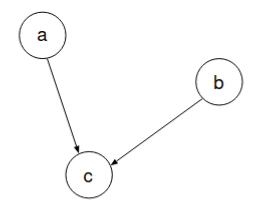
\includegraphics[width=0.3\textwidth]{images/red_bayesiana_simple.png}
    \caption{Ejemplo de red bayesiana}
\end{figure}

\subsection{Idependencia condicional}

Se dice que $a$ es incondicionalmente independiente de $b$, y se denota
como $a \perp b$, si y solo si

$$ P(a, b) = P(a) P(b) $$
$$ P(a|b) = P(a) $$

Se dice que $a$ es condicionalmente independiente de $b$ dado $c$, y se
denota como $a \perp b | c$, si y solo si

$$ P(a, b|c) = P(a|c) P(b|c) $$
$$ P(a|b, c) = P(a|c) $$

\subsubsection{Reglas de independencia condicional e incondicional}

\textbf{Dirección causal}: $(a \perp b | c) \quad (a \cancel{\perp} b )$

$$ P(a, b|c) = \frac{P(a, b, c)}{P(c)} = \frac{P(a|c) P(b|c) P(c)}{P(c)} = P(a|c) P(b|c) $$

pero en general $P(a, b) \neq P(a) P(b)$

\textbf{Causa común}: $ (a \perp b | c) \quad (a \cancel{\perp} b) $

$$ P(a, b|c) = \frac{P(a, b, c)}{P(c)} = \frac{P(a|c) P(b|c) P(c)}{P(c)} = P(a|c) P(b|c) $$

pero en general $P(a, b) \neq P(a) P(b)$

\textbf{Estructura en V}: $ (a \cancel{\perp} b) \quad (a \perp b | c) $

$$ P(a, b|c) \neq P(a|c) P(b|c) $$

pero 

$$ P(a, b) = \sum_c P(a, b, c) = \sum_c P(a) P(b) P(c | a, b) = P(a) P(b) $$

\subsection{Inferencia con Redes Bayesianas}

En general, el problema consiste en calcular la probabilidad a posteriori
de alguna variable $x$ a partir de las distribuciones conjuntas asociadas
a una red bayesiana, dada alguna evidencia $e$ (como valores de otras variables)
y sin importar el resto de las variables $f$.

\[
P(x \mid e) = \frac{P(x, e)}{P(e)} \quad \text{con:} \quad
P(x, e) = \sum_f P(x, e, f); \quad
P(e) = \sum_{x, f} P(x, e, f)
\]

El objetivo es calcular eficientemente $P(x, e) y P(e)$.

\begin{exercisebox}{Ejercicio ejemplo}
    Ejercicio de la página 14 de las diapositivas.
\end{exercisebox}

$ A = f $, $L = n$, $C = m$

\begin{align*}
P(A = f | L = n, C = m) = \frac{P(A = f, L = n, C = m)}{P(L = n, C = m)} = \\[1em]
\frac{P(L = n) P(A = f | L = n) P(C = n | L = n, A = f)}{\sum_{a = \{p, f\}} P(A=a, L=n, C=m)} = \\[1em]
\frac{0.8 \cdot 0.4 \cdot 0.9}{0.288 + (0.8 \cdot 0.6 \cdot 0.01)} = \frac{0.288}{0.288 + 0.0048} = \frac{0.288}{0.2948} = 0.9836
\end{align*}

\begin{exercisebox}{Apartado B del mismo ejemplo}
    No llueve, cuál es la mejor predicción sobre el estado del césped?
\end{exercisebox}

$$ \text{argmax}_{c \in \{r, m\}} P(C = c | L = n) $$

$$ P(C = c | L = n) = \frac{P(C = r, L = n)}{P(L = n)}$$

Como $P(L = n)$ no depende de $c$, podemos ignorarla si queremos saber el máximo.

$$P(C = r, L = n) = \sum_{a \in \{p, f\}} P(C = r, L = n, A = a)$$

Para $c = r$:

\begin{align*}
    P(C = r, L = n, A = f) + P(C = r, L = n, A = p) = \\[1em]
    P(L = n) P(A = p | L = n) P(C = r | L = n, A = p) + P(L = n) P(A = f | L = n) P(C = r | L = n, A = f) = \\[1em]
    (0.8 \cdot 0.6 \cdot 0.99) + (0.8 \cdot 0.4 \cdot 0.1) = 0.4752 + 0.032 = 0.5072
\end{align*}

Para calcular la probabilidad, dividimos por $P(L = n)$

$$ P(C = r | L = n) = \frac{0.5072}{0.8} = 0.634 $$

Como solo hay dos casos, $P(C = m | L = n) = 1 - 0.634 = 0.366$

Por lo tanto, la mejor predicción es que el césped esté reseco.

\begin{exercisebox}{Ejemplo del cáncer}
    ¿Cuál es la probabilidad de que un paciente no fumador no tenga cáncer si
    la radiografía ha dado un resultado negativo pero sufre de disnea?
\end{exercisebox}

Nos piden $ P(C = n | F = n, X = n, D = s) $

\begin{align*}
    P(C = n | F = n, X = n, D = s) = \frac{P(C = n, F = n, X = n, D = s)}{P(F = n, X = n, D = s)} = \\[1em]
    \frac{\sum_{p \in \{b, a\}} P(C = n, F = n, X = n, D = s, P = p)}{\sum_{c \in \{n, p\}} \sum_{p \in \{b, a\}} P(C = c, F = n, X = n, D = s, P = p)}
\end{align*}

Para simplificar, la forma de calcular $P(C, F, X, D, P)$ es

$$ P(C, F, X, D, P) = P(P) \cdot P(F) \cdot P(C | P, F) \cdot P(X | C) \cdot P(D | C) $$

\begin{exercisebox}{Ejercicio de examen sobre el cáncer}
    ¿Cuál es la mejor predicción sobre el cáncer si el paciente es fumador,
    sufre disnea y el resultado de la radiografía ha sido dudoso? Proporcione
    la probabilidad de cada una.
\end{exercisebox}

Nos piden $\text{argmax} c \in \{n, s\} P(C = c | F = f, X = d, D = s)$

\begin{align*}
    P(C = c | F = f, X = d, D = s) = \frac{P(C = c, F = f, X = d, D = s)}{P(F = f, X = d, D = s)} = \\[1em]
    \frac{\sum_{p \in \{b, a\}} P(C = c, F = f, X = d, D = s, P = p)}{\sum_{c \in \{n, p\}} \sum_{p \in \{b, a\}} P(C = c, F = f, X = d, D = s, P = p)}
\end{align*}

Podemos simplificar la fórmula quitando el denominador, ya que no
depende de $c$ y solo queremos el máximo.

\begin{align*}
    \sum_{p \in \{b, a\}} P(C = c, F = f, X = d, D = s, P = p) = \\[1em]
    \sum_{p \in \{b, a\}} P(P = p) \cdot P(F = f) \cdot P(C = c | P = p, F = f) \cdot P(X = d | C = c) P(D = s | C = c) = \\[1em]
\end{align*}

El ejercicio está resuelto en el pdf del examen.
